\section{Layer~15 – Responsible Recursive Morphogenesis}
\label{sec:layer15}

% ----- SUPERKRACHT -----
\begin{tcolorbox}[colback=blue!5, colframe=blue!60, title=\textbf{Superpower: The Sculptor}]
\begin{center}
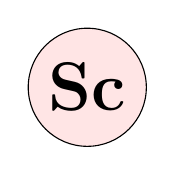
\begin{tikzpicture}
  \node[draw, circle, fill=red!10, minimum size=1.5cm, font=\bfseries\Huge] {Sc};
\end{tikzpicture}
\textit{“How do I safely change the real world?”}
\end{center}
\end{tcolorbox}

Until now Pixel lived in a digital world.  Layer~15 is the
\textbf{bridge to physical reality}: it enables Pixel to propose
changing real materials – for example, controlling a 3D printer or
moving the rover’s robot arm.

\begin{tcolorbox}[colback=yellow!5, colframe=yellow!80, title=Real‑life analogy]
A surgeon controlling a robot remotely must be 100\% sure every
movement is safe.  There is an “emergency stop” and every step is
verified.  Pixel’s Layer~15 has such an emergency stop built in.
\end{tcolorbox}

\textbf{Irreversibility requires permission.}
Pixel may only carry out actions that can be undone.  If it wants to
do something permanent – like drilling a hole in the rover – a human
council must first give consent.  This \textbf{built‑in ethical
compass} prevents a super‑intelligent machine from ever making large,
irreversible changes without permission.